\documentclass[]{article}
\usepackage{lmodern}
\usepackage{amssymb,amsmath}
\usepackage{ifxetex,ifluatex}
\usepackage{fixltx2e} % provides \textsubscript
\ifnum 0\ifxetex 1\fi\ifluatex 1\fi=0 % if pdftex
  \usepackage[T1]{fontenc}
  \usepackage[utf8]{inputenc}
\else % if luatex or xelatex
  \ifxetex
    \usepackage{mathspec}
  \else
    \usepackage{fontspec}
  \fi
  \defaultfontfeatures{Ligatures=TeX,Scale=MatchLowercase}
\fi
% use upquote if available, for straight quotes in verbatim environments
\IfFileExists{upquote.sty}{\usepackage{upquote}}{}
% use microtype if available
\IfFileExists{microtype.sty}{%
\usepackage{microtype}
\UseMicrotypeSet[protrusion]{basicmath} % disable protrusion for tt fonts
}{}
\usepackage[margin=1in]{geometry}
\usepackage{hyperref}
\hypersetup{unicode=true,
            pdftitle={Practical Machine Learning: Project},
            pdfauthor={Manojkumar Parmar},
            pdfborder={0 0 0},
            breaklinks=true}
\urlstyle{same}  % don't use monospace font for urls
\usepackage{color}
\usepackage{fancyvrb}
\newcommand{\VerbBar}{|}
\newcommand{\VERB}{\Verb[commandchars=\\\{\}]}
\DefineVerbatimEnvironment{Highlighting}{Verbatim}{commandchars=\\\{\}}
% Add ',fontsize=\small' for more characters per line
\usepackage{framed}
\definecolor{shadecolor}{RGB}{248,248,248}
\newenvironment{Shaded}{\begin{snugshade}}{\end{snugshade}}
\newcommand{\KeywordTok}[1]{\textcolor[rgb]{0.13,0.29,0.53}{\textbf{{#1}}}}
\newcommand{\DataTypeTok}[1]{\textcolor[rgb]{0.13,0.29,0.53}{{#1}}}
\newcommand{\DecValTok}[1]{\textcolor[rgb]{0.00,0.00,0.81}{{#1}}}
\newcommand{\BaseNTok}[1]{\textcolor[rgb]{0.00,0.00,0.81}{{#1}}}
\newcommand{\FloatTok}[1]{\textcolor[rgb]{0.00,0.00,0.81}{{#1}}}
\newcommand{\ConstantTok}[1]{\textcolor[rgb]{0.00,0.00,0.00}{{#1}}}
\newcommand{\CharTok}[1]{\textcolor[rgb]{0.31,0.60,0.02}{{#1}}}
\newcommand{\SpecialCharTok}[1]{\textcolor[rgb]{0.00,0.00,0.00}{{#1}}}
\newcommand{\StringTok}[1]{\textcolor[rgb]{0.31,0.60,0.02}{{#1}}}
\newcommand{\VerbatimStringTok}[1]{\textcolor[rgb]{0.31,0.60,0.02}{{#1}}}
\newcommand{\SpecialStringTok}[1]{\textcolor[rgb]{0.31,0.60,0.02}{{#1}}}
\newcommand{\ImportTok}[1]{{#1}}
\newcommand{\CommentTok}[1]{\textcolor[rgb]{0.56,0.35,0.01}{\textit{{#1}}}}
\newcommand{\DocumentationTok}[1]{\textcolor[rgb]{0.56,0.35,0.01}{\textbf{\textit{{#1}}}}}
\newcommand{\AnnotationTok}[1]{\textcolor[rgb]{0.56,0.35,0.01}{\textbf{\textit{{#1}}}}}
\newcommand{\CommentVarTok}[1]{\textcolor[rgb]{0.56,0.35,0.01}{\textbf{\textit{{#1}}}}}
\newcommand{\OtherTok}[1]{\textcolor[rgb]{0.56,0.35,0.01}{{#1}}}
\newcommand{\FunctionTok}[1]{\textcolor[rgb]{0.00,0.00,0.00}{{#1}}}
\newcommand{\VariableTok}[1]{\textcolor[rgb]{0.00,0.00,0.00}{{#1}}}
\newcommand{\ControlFlowTok}[1]{\textcolor[rgb]{0.13,0.29,0.53}{\textbf{{#1}}}}
\newcommand{\OperatorTok}[1]{\textcolor[rgb]{0.81,0.36,0.00}{\textbf{{#1}}}}
\newcommand{\BuiltInTok}[1]{{#1}}
\newcommand{\ExtensionTok}[1]{{#1}}
\newcommand{\PreprocessorTok}[1]{\textcolor[rgb]{0.56,0.35,0.01}{\textit{{#1}}}}
\newcommand{\AttributeTok}[1]{\textcolor[rgb]{0.77,0.63,0.00}{{#1}}}
\newcommand{\RegionMarkerTok}[1]{{#1}}
\newcommand{\InformationTok}[1]{\textcolor[rgb]{0.56,0.35,0.01}{\textbf{\textit{{#1}}}}}
\newcommand{\WarningTok}[1]{\textcolor[rgb]{0.56,0.35,0.01}{\textbf{\textit{{#1}}}}}
\newcommand{\AlertTok}[1]{\textcolor[rgb]{0.94,0.16,0.16}{{#1}}}
\newcommand{\ErrorTok}[1]{\textcolor[rgb]{0.64,0.00,0.00}{\textbf{{#1}}}}
\newcommand{\NormalTok}[1]{{#1}}
\usepackage{longtable,booktabs}
\usepackage{graphicx,grffile}
\makeatletter
\def\maxwidth{\ifdim\Gin@nat@width>\linewidth\linewidth\else\Gin@nat@width\fi}
\def\maxheight{\ifdim\Gin@nat@height>\textheight\textheight\else\Gin@nat@height\fi}
\makeatother
% Scale images if necessary, so that they will not overflow the page
% margins by default, and it is still possible to overwrite the defaults
% using explicit options in \includegraphics[width, height, ...]{}
\setkeys{Gin}{width=\maxwidth,height=\maxheight,keepaspectratio}
\IfFileExists{parskip.sty}{%
\usepackage{parskip}
}{% else
\setlength{\parindent}{0pt}
\setlength{\parskip}{6pt plus 2pt minus 1pt}
}
\setlength{\emergencystretch}{3em}  % prevent overfull lines
\providecommand{\tightlist}{%
  \setlength{\itemsep}{0pt}\setlength{\parskip}{0pt}}
\setcounter{secnumdepth}{5}
% Redefines (sub)paragraphs to behave more like sections
\ifx\paragraph\undefined\else
\let\oldparagraph\paragraph
\renewcommand{\paragraph}[1]{\oldparagraph{#1}\mbox{}}
\fi
\ifx\subparagraph\undefined\else
\let\oldsubparagraph\subparagraph
\renewcommand{\subparagraph}[1]{\oldsubparagraph{#1}\mbox{}}
\fi

%%% Use protect on footnotes to avoid problems with footnotes in titles
\let\rmarkdownfootnote\footnote%
\def\footnote{\protect\rmarkdownfootnote}

%%% Change title format to be more compact
\usepackage{titling}

% Create subtitle command for use in maketitle
\newcommand{\subtitle}[1]{
  \posttitle{
    \begin{center}\large#1\end{center}
    }
}

\setlength{\droptitle}{-2em}
  \title{Practical Machine Learning: Project}
  \pretitle{\vspace{\droptitle}\centering\huge}
  \posttitle{\par}
  \author{Manojkumar Parmar}
  \preauthor{\centering\large\emph}
  \postauthor{\par}
  \predate{\centering\large\emph}
  \postdate{\par}
  \date{11/21/2016}


\begin{document}
\maketitle

{
\setcounter{tocdepth}{6}
\tableofcontents
}
\section{About Data}\label{about-data}

\subsection{Background}\label{background}

Using devices such as Jawbone Up, Nike FuelBand, and Fitbit it is now
possible to collect a large amount of data about personal activity
relatively inexpensively. These type of devices are part of the
quantified self movement -- a group of enthusiasts who take measurements
about themselves regularly to improve their health, to find patterns in
their behavior, or because they are tech geeks. One thing that people
regularly do is quantify how much of a particular activity they do, but
they rarely quantify how well they do it. In this project, your goal
will be to use data from accelerometers on the belt, forearm, arm, and
dumbell of 6 participants. They were asked to perform barbell lifts
correctly and incorrectly in 5 different ways. More information is
available from the website here:
\url{http://groupware.les.inf.puc-rio.br/har} (see the section on the
Weight Lifting Exercise Dataset).

\subsection{Data}\label{data}

The training data for this project are available here:
\url{https://d396qusza40orc.cloudfront.net/predmachlearn/pml-training.csv}
The test data are available here:
\url{https://d396qusza40orc.cloudfront.net/predmachlearn/pml-testing.csv}
The data for this project come from this source:
\url{http://groupware.les.inf.puc-rio.br/har}. If you use the document
you create for this class for any purpose please cite them as they have
been very generous in allowing their data to be used for this kind of
assignment.

\subsection{Goal of the Analysis}\label{goal-of-the-analysis}

The goal of your project is to predict the manner in which they did the
exercise. This is the ``classe'' variable in the training set. You may
use any of the other variables to predict with. You should create a
report describing how you built your model, how you used cross
validation, what you think the expected out of sample error is, and why
you made the choices you did. You will also use your prediction model to
predict 20 different test cases.

\subsubsection{Peer Review Portion}\label{peer-review-portion}

Your submission for the Peer Review portion should consist of a link to
a Github repo with your R markdown and compiled HTML file describing
your analysis. Please constrain the text of the writeup to \textless{}
2000 words and the number of figures to be less than 5. It will make it
easier for the graders if you submit a repo with a gh-pages branch so
the HTML page can be viewed online (and you always want to make it easy
on graders :-).

\section{Data Cleaning \& Basic
analysis}\label{data-cleaning-basic-analysis}

\subsection{Getting Data}\label{getting-data}

This method uses the URL provided to download files for training \& test
data.

\begin{Shaded}
\begin{Highlighting}[]
\NormalTok{if(!}\KeywordTok{file.exists}\NormalTok{(}\StringTok{"./projectdata"}\NormalTok{))\{}
        \KeywordTok{dir.create}\NormalTok{(}\StringTok{"./projectdata"}\NormalTok{)}
\NormalTok{\}}
\NormalTok{downloadUrlTrain <-}\StringTok{ "https://d396qusza40orc.cloudfront.net/predmachlearn/pml-training.csv"}
\NormalTok{if(!}\KeywordTok{file.exists}\NormalTok{(}\StringTok{"./projectdata/pml-training.csv"}\NormalTok{))\{}
        \KeywordTok{download.file}\NormalTok{(downloadUrlTrain,}\DataTypeTok{destfile=}\StringTok{"./projectdata/pml-training.csv"}\NormalTok{,}\DataTypeTok{method=}\StringTok{"curl"}\NormalTok{)}
\NormalTok{\}}
\NormalTok{downloadUrlTest <-}\StringTok{ "https://d396qusza40orc.cloudfront.net/predmachlearn/pml-testing.csv"}
\NormalTok{if(!}\KeywordTok{file.exists}\NormalTok{(}\StringTok{"./projectdata/pml-testing.csv"}\NormalTok{))\{}
        \KeywordTok{download.file}\NormalTok{(downloadUrlTest,}\DataTypeTok{destfile=}\StringTok{"./projectdata/pml-testing.csv"}\NormalTok{,}\DataTypeTok{method=}\StringTok{"curl"}\NormalTok{)}
\NormalTok{\}}
\end{Highlighting}
\end{Shaded}

\subsection{cleaning Data}\label{cleaning-data}

This method loads the data and cleans it. All the columns with
\textbf{all missing values} are discarded. Same way \textbf{first 7
columns} are not helpful for prediction purpose and hence they are
removed.

\begin{Shaded}
\begin{Highlighting}[]
\NormalTok{trainData <-}\StringTok{ }\KeywordTok{read.csv}\NormalTok{(}\StringTok{"./projectdata/pml-training.csv"}\NormalTok{, }
                      \DataTypeTok{na.strings =} \KeywordTok{c}\NormalTok{(}\StringTok{"NA"}\NormalTok{,}\StringTok{"#DIV/0!"}\NormalTok{, }\StringTok{""}\NormalTok{))}
\NormalTok{testData <-}\StringTok{ }\KeywordTok{read.csv}\NormalTok{(}\StringTok{"./projectdata/pml-testing.csv"}\NormalTok{,}
                     \DataTypeTok{na.strings =} \KeywordTok{c}\NormalTok{(}\StringTok{"NA"}\NormalTok{,}\StringTok{"#DIV/0!"}\NormalTok{, }\StringTok{""}\NormalTok{))}
\CommentTok{# delete colums with all missing values}
\NormalTok{trainData <-}\StringTok{ }\NormalTok{trainData[,}\KeywordTok{colSums}\NormalTok{(}\KeywordTok{is.na}\NormalTok{(trainData))==}\DecValTok{0}\NormalTok{]}
\NormalTok{testData <-}\StringTok{ }\NormalTok{testData[,}\KeywordTok{colSums}\NormalTok{(}\KeywordTok{is.na}\NormalTok{(testData))==}\DecValTok{0}\NormalTok{]}
\CommentTok{# remove unnecesary data as it is not relavant}
\NormalTok{trainData <-}\StringTok{ }\NormalTok{trainData[,-}\KeywordTok{c}\NormalTok{(}\DecValTok{1}\NormalTok{:}\DecValTok{7}\NormalTok{)]}
\NormalTok{testData <-}\StringTok{ }\NormalTok{testData[,-}\KeywordTok{c}\NormalTok{(}\DecValTok{1}\NormalTok{:}\DecValTok{7}\NormalTok{)]}
\end{Highlighting}
\end{Shaded}

\subsection{Generating training, testing \& validation
data}\label{generating-training-testing-validation-data}

This method divides training data in to \textbf{training} part
(\(60\)\%), \textbf{testing} part (\(20\)\%) \& \textbf{validation} part
(\(20\)\%)

\begin{Shaded}
\begin{Highlighting}[]
\KeywordTok{set.seed}\NormalTok{(}\DecValTok{123}\NormalTok{)}
\NormalTok{inBuild <-}\StringTok{ }\KeywordTok{createDataPartition}\NormalTok{(}\DataTypeTok{y =} \NormalTok{trainData$classe, }\DataTypeTok{p =} \FloatTok{0.8}\NormalTok{, }\DataTypeTok{list =} \NormalTok{F)}
\NormalTok{buildData <-}\StringTok{ }\NormalTok{trainData[inBuild,]}
\NormalTok{validation <-}\StringTok{ }\NormalTok{trainData[-inBuild,]}
\NormalTok{inTrain <-}\StringTok{ }\KeywordTok{createDataPartition}\NormalTok{(}\DataTypeTok{y =} \NormalTok{buildData$classe, }\DataTypeTok{p =} \FloatTok{0.75}\NormalTok{, }\DataTypeTok{list =} \NormalTok{F)}
\NormalTok{training <-}\StringTok{ }\NormalTok{buildData[inTrain,]}
\NormalTok{testing <-}\StringTok{ }\NormalTok{buildData[-inTrain,]}
\end{Highlighting}
\end{Shaded}

Here are the dimensions of various subsets after split

\begin{Shaded}
\begin{Highlighting}[]
\KeywordTok{dim}\NormalTok{(validation)}
\end{Highlighting}
\end{Shaded}

\begin{verbatim}
## [1] 3923   53
\end{verbatim}

\begin{Shaded}
\begin{Highlighting}[]
\KeywordTok{dim}\NormalTok{(training)}
\end{Highlighting}
\end{Shaded}

\begin{verbatim}
## [1] 11776    53
\end{verbatim}

\begin{Shaded}
\begin{Highlighting}[]
\KeywordTok{dim}\NormalTok{(testing)}
\end{Highlighting}
\end{Shaded}

\begin{verbatim}
## [1] 3923   53
\end{verbatim}

\subsection{Exploration of data}\label{exploration-of-data}

Exploration of predicted variable ``\textbf{classe}'' reveals that it is
\emph{uniform} in nature \& hence model based analysis will yield poor
results.

\begin{Shaded}
\begin{Highlighting}[]
\KeywordTok{qplot}\NormalTok{(classe,}\DataTypeTok{data=}\NormalTok{training, }\DataTypeTok{main=}\StringTok{"Distribution of Classes"}\NormalTok{)}
\end{Highlighting}
\end{Shaded}

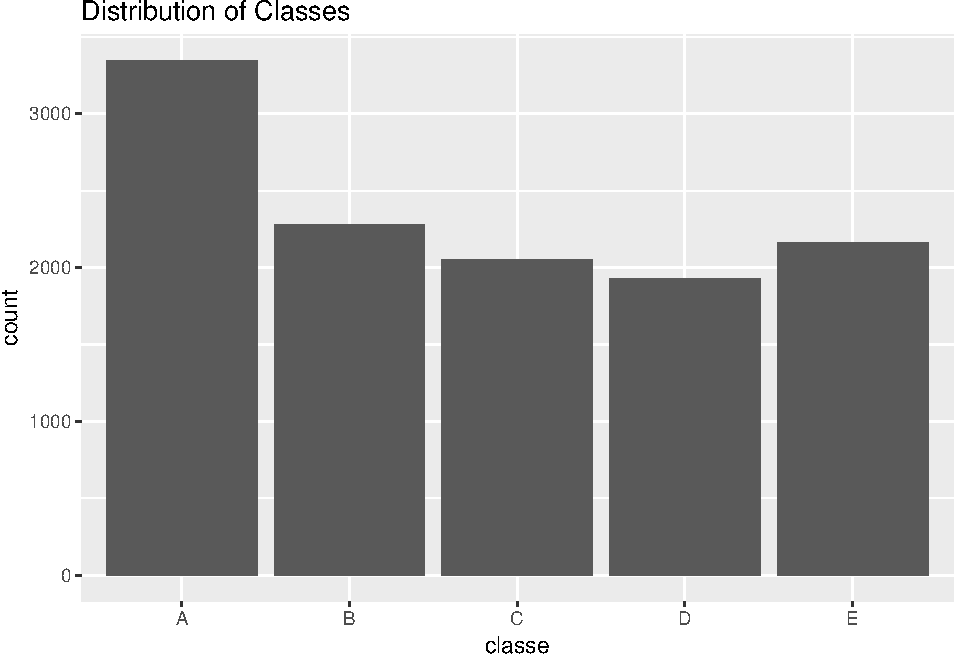
\includegraphics{index_files/figure-latex/unnamed-chunk-6-1.pdf}

There exist a \textbf{very high corelation} (\textgreater{} \(0.8\))
between predictors and hence ``\textbf{pca}''\$ needs to be used as
preprocessor step.

\begin{Shaded}
\begin{Highlighting}[]
\CommentTok{#find correlation}
\NormalTok{highCor <-}\StringTok{ }\KeywordTok{findCorrelation}\NormalTok{(}\KeywordTok{cor}\NormalTok{(training[,-}\DecValTok{53}\NormalTok{]), }\DataTypeTok{cutoff =} \FloatTok{0.8}\NormalTok{)}
\KeywordTok{names}\NormalTok{(training)[highCor]}
\end{Highlighting}
\end{Shaded}

\begin{verbatim}
##  [1] "accel_belt_z"     "roll_belt"        "accel_belt_y"    
##  [4] "accel_dumbbell_z" "accel_belt_x"     "magnet_belt_x"   
##  [7] "accel_arm_x"      "accel_dumbbell_x" "magnet_arm_y"    
## [10] "magnet_belt_z"    "gyros_forearm_y"  "gyros_dumbbell_x"
## [13] "gyros_dumbbell_z" "gyros_arm_x"
\end{verbatim}

Following are \textbf{list of predictors} which are used to build model.

\begin{Shaded}
\begin{Highlighting}[]
\CommentTok{#final predictors}
\KeywordTok{names}\NormalTok{(training[,-}\DecValTok{53}\NormalTok{])}
\end{Highlighting}
\end{Shaded}

\begin{verbatim}
##  [1] "roll_belt"            "pitch_belt"           "yaw_belt"            
##  [4] "total_accel_belt"     "gyros_belt_x"         "gyros_belt_y"        
##  [7] "gyros_belt_z"         "accel_belt_x"         "accel_belt_y"        
## [10] "accel_belt_z"         "magnet_belt_x"        "magnet_belt_y"       
## [13] "magnet_belt_z"        "roll_arm"             "pitch_arm"           
## [16] "yaw_arm"              "total_accel_arm"      "gyros_arm_x"         
## [19] "gyros_arm_y"          "gyros_arm_z"          "accel_arm_x"         
## [22] "accel_arm_y"          "accel_arm_z"          "magnet_arm_x"        
## [25] "magnet_arm_y"         "magnet_arm_z"         "roll_dumbbell"       
## [28] "pitch_dumbbell"       "yaw_dumbbell"         "total_accel_dumbbell"
## [31] "gyros_dumbbell_x"     "gyros_dumbbell_y"     "gyros_dumbbell_z"    
## [34] "accel_dumbbell_x"     "accel_dumbbell_y"     "accel_dumbbell_z"    
## [37] "magnet_dumbbell_x"    "magnet_dumbbell_y"    "magnet_dumbbell_z"   
## [40] "roll_forearm"         "pitch_forearm"        "yaw_forearm"         
## [43] "total_accel_forearm"  "gyros_forearm_x"      "gyros_forearm_y"     
## [46] "gyros_forearm_z"      "accel_forearm_x"      "accel_forearm_y"     
## [49] "accel_forearm_z"      "magnet_forearm_x"     "magnet_forearm_y"    
## [52] "magnet_forearm_z"
\end{verbatim}

\section{Model Building}\label{model-building}

\subsection{trainControl Parameter}\label{traincontrol-parameter}

Following training parameters are used for the model building.

\begin{itemize}
\tightlist
\item
  \textbf{Cross validation} method is used with \textbf{7 folds}
\item
  \textbf{Principle component analysis} is used as pre processing step
\item
  Parallel processing is allowed to build model
\end{itemize}

\begin{Shaded}
\begin{Highlighting}[]
\CommentTok{# train control parameter}
\NormalTok{fitCtrl <-}\StringTok{ }\KeywordTok{trainControl}\NormalTok{(}\DataTypeTok{method =} \StringTok{"cv"}\NormalTok{,}\DataTypeTok{number =} \DecValTok{7}\NormalTok{, }\DataTypeTok{verboseIter =} \NormalTok{F, }
                        \DataTypeTok{preProcOptions =} \KeywordTok{c}\NormalTok{(}\StringTok{"pca"}\NormalTok{),}
                        \DataTypeTok{allowParallel =} \NormalTok{T)}
\end{Highlighting}
\end{Shaded}

\subsection{Model Selection}\label{model-selection}

Model selection is carried out by \textbf{building multiple models} and
later selecting best performing models based on \textbf{average
accuracy}. \emph{Gradient boosting, random forest, support vector
machine radial, support vecor machine linear, neuralnet \& logit boost}
are primary candidates.

\subsubsection{Evaluating multiple
models}\label{evaluating-multiple-models}

Models are build \(10\) times and their respective accuracy is captured
for all run.

\begin{Shaded}
\begin{Highlighting}[]
\CommentTok{# generate dataframe over multiple prediction}
\NormalTok{predDf <-}\StringTok{ }\KeywordTok{data.frame}\NormalTok{(}\DataTypeTok{run =} \DecValTok{0}\NormalTok{, }\DataTypeTok{time =} \DecValTok{0}\NormalTok{, }\DataTypeTok{gbm =} \DecValTok{0}\NormalTok{, }\DataTypeTok{rf =} \DecValTok{0}\NormalTok{, }\DataTypeTok{svmr =} \DecValTok{0}\NormalTok{, }
                     \DataTypeTok{svml =} \DecValTok{0}\NormalTok{, }\DataTypeTok{nn =} \DecValTok{0}\NormalTok{, }\DataTypeTok{lb =} \DecValTok{0}\NormalTok{)}
\NormalTok{start.time.all =}\StringTok{ }\KeywordTok{Sys.time}\NormalTok{() }\CommentTok{#log the starting time}
\CommentTok{# Run the model buiding 10 times & record accuracy over test set}
\NormalTok{for (i in }\DecValTok{1}\NormalTok{:}\DecValTok{10}\NormalTok{)\{}
        \NormalTok{inTrain <-}\StringTok{ }\KeywordTok{createDataPartition}\NormalTok{(}\DataTypeTok{y =} \NormalTok{buildData$classe, }\DataTypeTok{p =} \FloatTok{0.75}\NormalTok{, }\DataTypeTok{list =} \NormalTok{F)}
        \NormalTok{training <-}\StringTok{ }\NormalTok{buildData[inTrain,]}
        \NormalTok{testing <-}\StringTok{ }\NormalTok{buildData[-inTrain,]}
        \KeywordTok{dim}\NormalTok{(validation)}
        \KeywordTok{dim}\NormalTok{(training)}
        \KeywordTok{dim}\NormalTok{(testing)}
        \CommentTok{#Start building model}
        \NormalTok{start.time =}\StringTok{ }\KeywordTok{Sys.time}\NormalTok{()}
        \NormalTok{mod.gbm <-}\StringTok{ }\KeywordTok{train}\NormalTok{(classe ~}\StringTok{ }\NormalTok{. , }\DataTypeTok{data=} \NormalTok{training , }\DataTypeTok{method =} \StringTok{"gbm"}\NormalTok{, }
                         \DataTypeTok{trControl =} \NormalTok{fitCtrl, }\DataTypeTok{verbose =} \NormalTok{F)}
        \NormalTok{mod.rf <-}\StringTok{ }\KeywordTok{train}\NormalTok{(classe ~}\StringTok{ }\NormalTok{. , }\DataTypeTok{data=} \NormalTok{training , }\DataTypeTok{method =} \StringTok{"rf"}\NormalTok{, }
                        \DataTypeTok{trControl =} \NormalTok{fitCtrl, }\DataTypeTok{verbose =} \NormalTok{F)}
        \NormalTok{mod.svmr <-}\StringTok{ }\KeywordTok{train}\NormalTok{(classe ~}\StringTok{ }\NormalTok{. , }\DataTypeTok{data=} \NormalTok{training , }\DataTypeTok{method =} \StringTok{"svmRadial"}\NormalTok{, }
                          \DataTypeTok{trControl =} \NormalTok{fitCtrl, }\DataTypeTok{verbose =} \NormalTok{F)}
        \NormalTok{mod.svml <-}\StringTok{ }\KeywordTok{train}\NormalTok{(classe ~}\StringTok{ }\NormalTok{. , }\DataTypeTok{data=} \NormalTok{training , }\DataTypeTok{method =} \StringTok{"svmLinear"}\NormalTok{, }
                         \DataTypeTok{trControl =} \NormalTok{fitCtrl, }\DataTypeTok{verbose =} \NormalTok{F)}
        \NormalTok{mod.nn <-}\StringTok{ }\KeywordTok{train}\NormalTok{(classe ~}\StringTok{ }\NormalTok{. , }\DataTypeTok{data=} \NormalTok{training , }\DataTypeTok{method =} \StringTok{"nnet"}\NormalTok{, }
                        \DataTypeTok{trControl =} \NormalTok{fitCtrl, }\DataTypeTok{verbose =} \NormalTok{F)}
        \NormalTok{mod.lb <-}\StringTok{ }\KeywordTok{train}\NormalTok{(classe ~}\StringTok{ }\NormalTok{. , }\DataTypeTok{data=} \NormalTok{training , }\DataTypeTok{method =} \StringTok{"LogitBoost"}\NormalTok{, }
                        \DataTypeTok{trControl =} \NormalTok{fitCtrl, }\DataTypeTok{verbose =} \NormalTok{F)}
        \NormalTok{stop.time =}\StringTok{ }\KeywordTok{Sys.time}\NormalTok{()}
        
        \CommentTok{#Predictions}
        \NormalTok{pred_val <-}\StringTok{ }\KeywordTok{c}\NormalTok{( i, (stop.time -}\StringTok{ }\NormalTok{start.time),}
                        \KeywordTok{unname}\NormalTok{(}\KeywordTok{confusionMatrix}\NormalTok{(}\KeywordTok{predict}\NormalTok{(mod.gbm, testing), }
                                               \NormalTok{testing$classe)$overall[}\DecValTok{1}\NormalTok{]),}
                        \KeywordTok{unname}\NormalTok{(}\KeywordTok{confusionMatrix}\NormalTok{(}\KeywordTok{predict}\NormalTok{(mod.rf, testing), }
                                               \NormalTok{testing$classe)$overall[}\DecValTok{1}\NormalTok{]),}
                        \KeywordTok{unname}\NormalTok{(}\KeywordTok{confusionMatrix}\NormalTok{(}\KeywordTok{predict}\NormalTok{(mod.svmr, testing), }
                                               \NormalTok{testing$classe)$overall[}\DecValTok{1}\NormalTok{]),}
                        \KeywordTok{unname}\NormalTok{(}\KeywordTok{confusionMatrix}\NormalTok{(}\KeywordTok{predict}\NormalTok{(mod.svml, testing), }
                                               \NormalTok{testing$classe)$overall[}\DecValTok{1}\NormalTok{]),}
                        \KeywordTok{unname}\NormalTok{(}\KeywordTok{confusionMatrix}\NormalTok{(}\KeywordTok{predict}\NormalTok{(mod.nn, testing), }
                                               \NormalTok{testing$classe)$overall[}\DecValTok{1}\NormalTok{]),}
                        \KeywordTok{unname}\NormalTok{(}\KeywordTok{confusionMatrix}\NormalTok{(}\KeywordTok{predict}\NormalTok{(mod.lb, testing), }
                                               \NormalTok{testing$classe)$overall[}\DecValTok{1}\NormalTok{]))}
        \NormalTok{predDf <-}\StringTok{ }\KeywordTok{rbind}\NormalTok{(predDf, pred_val)}
\NormalTok{\}}
\NormalTok{stop.time.all =}\StringTok{ }\KeywordTok{Sys.time}\NormalTok{()}
\CommentTok{#calculate total time for execution}
\KeywordTok{print}\NormalTok{(stop.time.all -}\StringTok{ }\NormalTok{start.time.all)}
\CommentTok{#correct the prediction frame}
\NormalTok{predDf <-}\StringTok{ }\NormalTok{predDf[-}\DecValTok{1}\NormalTok{,]}
\end{Highlighting}
\end{Shaded}

\subsubsection{Accuracy of multiple
models}\label{accuracy-of-multiple-models}

Following shows the \textbf{accuracy} of all models for \textbf{all
runs}. Please note that models are refereed by short names.

\begin{Shaded}
\begin{Highlighting}[]
\KeywordTok{rownames}\NormalTok{(predDf) <-}\StringTok{ }\OtherTok{NULL}
\KeywordTok{kable}\NormalTok{(predDf[,-}\KeywordTok{c}\NormalTok{(}\DecValTok{2}\NormalTok{)], }\DataTypeTok{digits =} \DecValTok{3}\NormalTok{)}
\end{Highlighting}
\end{Shaded}

\begin{longtable}[]{@{}rrrrrrr@{}}
\toprule
run & gbm & rf & svmr & svml & nn & lb\tabularnewline
\midrule
\endhead
1 & 0.963 & 0.993 & 0.916 & 0.783 & 0.401 & 0.909\tabularnewline
2 & 0.958 & 0.992 & 0.925 & 0.788 & 0.441 & 0.893\tabularnewline
3 & 0.962 & 0.990 & 0.922 & 0.782 & 0.429 & 0.900\tabularnewline
4 & 0.958 & 0.993 & 0.923 & 0.771 & 0.403 & 0.887\tabularnewline
5 & 0.963 & 0.993 & 0.925 & 0.780 & 0.420 & 0.896\tabularnewline
6 & 0.954 & 0.988 & 0.923 & 0.778 & 0.401 & 0.894\tabularnewline
7 & 0.959 & 0.991 & 0.924 & 0.781 & 0.465 & 0.898\tabularnewline
8 & 0.956 & 0.988 & 0.914 & 0.773 & 0.500 & 0.890\tabularnewline
9 & 0.959 & 0.991 & 0.913 & 0.776 & 0.396 & 0.877\tabularnewline
10 & 0.964 & 0.992 & 0.921 & 0.784 & 0.369 & 0.889\tabularnewline
\bottomrule
\end{longtable}

\textbf{Average accuracy} of all runs for all models are as per
following

\begin{Shaded}
\begin{Highlighting}[]
\NormalTok{modAccuracy <-}\StringTok{ }\KeywordTok{data.frame}\NormalTok{(}\KeywordTok{colMeans}\NormalTok{(predDf[,-}\KeywordTok{c}\NormalTok{(}\DecValTok{1}\NormalTok{,}\DecValTok{2}\NormalTok{)]))}
\KeywordTok{colnames}\NormalTok{(modAccuracy) <-}\StringTok{ "Avg. Accuracy"}
\KeywordTok{kable}\NormalTok{(}\KeywordTok{t}\NormalTok{(modAccuracy), }\DataTypeTok{digits =} \DecValTok{3}\NormalTok{)}
\end{Highlighting}
\end{Shaded}

\begin{longtable}[]{@{}lrrrrrr@{}}
\toprule
& gbm & rf & svmr & svml & nn & lb\tabularnewline
\midrule
\endhead
Avg. Accuracy & 0.96 & 0.991 & 0.92 & 0.78 & 0.422 &
0.893\tabularnewline
\bottomrule
\end{longtable}

From average accuracy point of view, \textbf{random forrest} is
\textbf{best} performing model. \emph{Gradient boosting} and
\emph{support vector machine radial} are respectively \emph{second} and
\emph{third} best model.

\subsubsection{Selection of final set of Models \& out of sample
accuracy}\label{selection-of-final-set-of-models-out-of-sample-accuracy}

Best models are used to predict values on \textbf{validation data set}
(only once) for calculation of ``\textbf{out of sample}'' accuracy.

\begin{Shaded}
\begin{Highlighting}[]
\NormalTok{validAccuracy <-}\StringTok{ }\KeywordTok{data.frame}\NormalTok{(}\DataTypeTok{Accuracy =} \KeywordTok{c}\NormalTok{(}
\KeywordTok{confusionMatrix}\NormalTok{(}\KeywordTok{predict}\NormalTok{(mod.rf, validation), validation$classe)$overall[}\DecValTok{1}\NormalTok{],}
\KeywordTok{confusionMatrix}\NormalTok{(}\KeywordTok{predict}\NormalTok{(mod.gbm, validation), validation$classe)$overall[}\DecValTok{1}\NormalTok{],}
\KeywordTok{confusionMatrix}\NormalTok{(}\KeywordTok{predict}\NormalTok{(mod.svmr, validation), validation$classe)$overall[}\DecValTok{1}\NormalTok{]))}
\KeywordTok{rownames}\NormalTok{(validAccuracy) <-}\StringTok{ }\KeywordTok{c}\NormalTok{(}\StringTok{"rf"}\NormalTok{, }\StringTok{"gbm"}\NormalTok{, }\StringTok{"svmr"}\NormalTok{)}
\KeywordTok{kable}\NormalTok{(}\KeywordTok{t}\NormalTok{(validAccuracy), }\DataTypeTok{digits =} \DecValTok{3}\NormalTok{)}
\end{Highlighting}
\end{Shaded}

\begin{longtable}[]{@{}lrrr@{}}
\toprule
& rf & gbm & svmr\tabularnewline
\midrule
\endhead
Accuracy & 0.991 & 0.962 & 0.918\tabularnewline
\bottomrule
\end{longtable}

From ``\textbf{out of sample}'' accuracy point of view, \textbf{random
forrest} is \textbf{best} performing model. \emph{Gradient boosting} and
\emph{support vector machine radial} are respectively \emph{second} and
\emph{third} best model.

Hence random forest is used for building final model.

\subsection{Final Model}\label{final-model}

\textbf{Random forest} model is built over \emph{original training
dataset}.

\begin{Shaded}
\begin{Highlighting}[]
\CommentTok{# Rf is best }
\NormalTok{finMod.rf <-}\StringTok{ }\KeywordTok{train}\NormalTok{(classe ~}\StringTok{ }\NormalTok{. , }\DataTypeTok{data=} \NormalTok{trainData , }\DataTypeTok{method =} \StringTok{"rf"}\NormalTok{, }
                \DataTypeTok{trControl =} \NormalTok{fitCtrl, }\DataTypeTok{verbose =} \NormalTok{F)}
\end{Highlighting}
\end{Shaded}

\subsection{Model agreement accuracy}\label{model-agreement-accuracy}

On original test set(\(20\) case), actual values are not available and
hence to improve prediction confidence level various \textbf{model
agreement accuracy} is used. Here additionally, gradient boosting and
support vector machine radial models are built on original training
dataset.

\begin{Shaded}
\begin{Highlighting}[]
\CommentTok{# gbm for agreement accuracy}
\NormalTok{finMod.gbm <-}\StringTok{ }\KeywordTok{train}\NormalTok{(classe ~}\StringTok{ }\NormalTok{. , }\DataTypeTok{data=} \NormalTok{trainData , }\DataTypeTok{method =} \StringTok{"gbm"}\NormalTok{, }
                   \DataTypeTok{trControl =} \NormalTok{fitCtrl, }\DataTypeTok{verbose =} \NormalTok{F)}

\CommentTok{#svmr for agreement accuracy}
\NormalTok{finMod.svmr <-}\StringTok{ }\KeywordTok{train}\NormalTok{(classe ~}\StringTok{ }\NormalTok{. , }\DataTypeTok{data=} \NormalTok{trainData , }\DataTypeTok{method =} \StringTok{"svmRadial"}\NormalTok{, }
                        \DataTypeTok{trControl =} \NormalTok{fitCtrl, }\DataTypeTok{verbose =} \NormalTok{F)}
\end{Highlighting}
\end{Shaded}

Prediction values are generated for all 3 models and used for checking
model agreement accuracy

\begin{Shaded}
\begin{Highlighting}[]
\CommentTok{#predict from 3 different best model}
\NormalTok{predFin.rf <-}\StringTok{ }\KeywordTok{predict}\NormalTok{(finMod.rf,testData)}
\NormalTok{predFin.gbm <-}\StringTok{ }\KeywordTok{predict}\NormalTok{(finMod.gbm,testData)}
\NormalTok{predFin.svmr <-}\StringTok{ }\KeywordTok{predict}\NormalTok{(finMod.svmr, testData)}
\CommentTok{#check for agreement accuracy}
\NormalTok{modAgreementAccuracy <-}\StringTok{ }\KeywordTok{data.frame}\NormalTok{(}\DataTypeTok{Agreement.Accuracy =} \KeywordTok{c}\NormalTok{(}
        \KeywordTok{confusionMatrix}\NormalTok{(predFin.gbm,predFin.rf)$overall[}\DecValTok{1}\NormalTok{],}
        \KeywordTok{confusionMatrix}\NormalTok{(predFin.svmr,predFin.rf)$overall[}\DecValTok{1}\NormalTok{]))}
\KeywordTok{rownames}\NormalTok{(modAgreementAccuracy) <-}\StringTok{ }\KeywordTok{c}\NormalTok{(}\StringTok{"gbm vs. rf"}\NormalTok{, }\StringTok{"svmr vs. rf"}\NormalTok{)}
\KeywordTok{kable}\NormalTok{(}\KeywordTok{t}\NormalTok{(modAgreementAccuracy), }\DataTypeTok{digits =} \DecValTok{3}\NormalTok{)}
\end{Highlighting}
\end{Shaded}

\begin{longtable}[]{@{}lrr@{}}
\toprule
& gbm vs.~rf & svmr vs.~rf\tabularnewline
\midrule
\endhead
Agreement.Accuracy & 1 & 1\tabularnewline
\bottomrule
\end{longtable}

Since all 3 models are in full agreement of predicted values, confidence
in \textbf{random forest} model is increased to very high level.

\section{Final prediction}\label{final-prediction}

Here is the final predicted values for test cases provided.

\begin{Shaded}
\begin{Highlighting}[]
\CommentTok{# Final prediction}
\NormalTok{finPred <-}\StringTok{ }\KeywordTok{data.frame}\NormalTok{(}\DataTypeTok{prediction =} \NormalTok{predFin.rf)}
\KeywordTok{rownames}\NormalTok{(finPred) <-}\StringTok{ }\DecValTok{1}\NormalTok{:}\KeywordTok{length}\NormalTok{(predFin.rf)}
\KeywordTok{kable}\NormalTok{(}\KeywordTok{t}\NormalTok{(finPred))}
\end{Highlighting}
\end{Shaded}

\begin{longtable}[]{@{}lllllllllllllllllllll@{}}
\toprule
& 1 & 2 & 3 & 4 & 5 & 6 & 7 & 8 & 9 & 10 & 11 & 12 & 13 & 14 & 15 & 16 &
17 & 18 & 19 & 20\tabularnewline
\midrule
\endhead
prediction & B & A & B & A & A & E & D & B & A & A & B & C & B & A & E &
E & A & B & B & B\tabularnewline
\bottomrule
\end{longtable}

\section{Reproducibility}\label{reproducibility}

Following is session-info to list respective packages along with their
versions

\begin{Shaded}
\begin{Highlighting}[]
\KeywordTok{sessionInfo}\NormalTok{()}
\end{Highlighting}
\end{Shaded}

\begin{verbatim}
## R version 3.3.2 (2016-10-31)
## Platform: x86_64-apple-darwin13.4.0 (64-bit)
## Running under: macOS Sierra 10.12.1
## 
## locale:
## [1] en_US.UTF-8/en_US.UTF-8/en_US.UTF-8/C/en_US.UTF-8/en_US.UTF-8
## 
## attached base packages:
## [1] splines   parallel  stats     graphics  grDevices utils     datasets 
## [8] methods   base     
## 
## other attached packages:
##  [1] kernlab_0.9-25      plyr_1.8.4          gbm_2.1.1          
##  [4] survival_2.40-1     doParallel_1.0.10   iterators_1.0.8    
##  [7] foreach_1.4.3       knitr_1.15          randomForest_4.6-12
## [10] caret_6.0-73        ggplot2_2.2.0       lattice_0.20-34    
## 
## loaded via a namespace (and not attached):
##  [1] Rcpp_0.12.8        highr_0.6          nloptr_1.0.4      
##  [4] class_7.3-14       tools_3.3.2        digest_0.6.10     
##  [7] lme4_1.1-12        evaluate_0.10      tibble_1.2        
## [10] nlme_3.1-128       gtable_0.2.0       mgcv_1.8-16       
## [13] Matrix_1.2-7.1     yaml_2.1.14        SparseM_1.74      
## [16] e1071_1.6-7        stringr_1.1.0      MatrixModels_0.4-1
## [19] stats4_3.3.2       grid_3.3.2         nnet_7.3-12       
## [22] rmarkdown_1.1      minqa_1.2.4        reshape2_1.4.2    
## [25] car_2.1-3          magrittr_1.5       scales_0.4.1      
## [28] codetools_0.2-15   ModelMetrics_1.1.0 htmltools_0.3.5   
## [31] MASS_7.3-45        assertthat_0.1     pbkrtest_0.4-6    
## [34] colorspace_1.3-1   labeling_0.3       quantreg_5.29     
## [37] stringi_1.1.2      lazyeval_0.2.0     munsell_0.4.3
\end{verbatim}

Hint : Majority of code here is executed separately and work space was
saved. Saved work space is used to create this report. Model selection
process is very time consuming (took on my machine 3.75 hr with parallel
processing enable).


\end{document}
